% USEFUL LINKS:
% -------------
%
% - UiO LaTeX guides:          https://www.mn.uio.no/ifi/tjenester/it/hjelp/latex/
% - Mathematics:               https://en.wikibooks.org/wiki/LaTeX/Mathematics
% - Physics:                   https://ctan.uib.no/macros/latex/contrib/physics/physics.pdf
% - Basics of Tikz:            https://en.wikibooks.org/wiki/LaTeX/PGF/Tikz
% - All the colors!            https://en.wikibooks.org/wiki/LaTeX/Colors
% - How to make tables:        https://en.wikibooks.org/wiki/LaTeX/Tables
% - Code listing styles:       https://en.wikibooks.org/wiki/LaTeX/Source_Code_Listings
% - \includegraphics           https://en.wikibooks.org/wiki/LaTeX/Importing_Graphics
% - Learn more about figures:  https://en.wikibooks.org/wiki/LaTeX/Floats,_Figures_and_Captions
% - Automagic bibliography:    https://en.wikibooks.org/wiki/LaTeX/Bibliography_Management  (this one is kinda difficult the first time)
%
%                              (This document is of class "revtex4-1", the REVTeX Guide explains how the class works)
%   REVTeX Guide:              http://www.physics.csbsju.edu/370/papers/Journal_Style_Manuals/auguide4-1.pdf
%
%
% COMPILING THE .pdf FILE IN THE LINUX TERMINAL
% ---------------------------------------------
%
% [terminal]$ pdflatex report_example.tex
%
% Run the command twice, always.
%
% When using references, footnotes, etc. you should run the following chain of commands:
%
% [terminal]$ pdflatex report_example.tex
% [terminal]$ bibtex report_example
% [terminal]$ pdflatex report_example.tex
% [terminal]$ pdflatex report_example.tex
%
% This series of commands can of course be gathered into a single-line command:
% [terminal]$ pdflatex report_example.tex && bibtex report_example.aux && pdflatex report_example.tex && pdflatex report_example.tex
%
% ----------------------------------------------------



% \documentclass[english,notitlepage,reprint,nofootinbib]{revtex4-2}  % defines the basic parameters of the document
\documentclass[english,notitlepage,reprint,nofootinbib]{revtex4-2}  % defines the basic parameters of the document
% If you want a single-column, remove "reprint"

% Allows special characters (including æøå)
\usepackage[utf8]{inputenc}
% \usepackage[english]{babel}

% Note that you may need to download some of these packages manually, it depends on your setup.
% It may be usefult to download TeXMaker, because it includes a large library of the most common packages.

\usepackage{physics,amssymb}  % mathematical symbols (physics imports amsmath)
\include{amsmath}
\usepackage{graphicx}         % include graphics such as plots
\usepackage{xcolor}           % set colors
\usepackage{hyperref}         % automagic cross-referencing
\usepackage{listings}         % display code
\usepackage{subfigure}        % imports a lot of cool and useful figure commands
% \usepackage{float}
%\usepackage[section]{placeins}
\usepackage{algorithm}
\usepackage[noend]{algpseudocode}
\usepackage{subfigure}
\usepackage{tikz}
\usepackage{cleveref}
\usepackage[version=4]{mhchem} % Correct package for writing out isotopes
\usetikzlibrary{quantikz}
% defines the color of hyperref objects
% Blending two colors:  blue!80!black  =  80% blue and 20% black
\hypersetup{ % this is just my personal choice, feel free to change things
    colorlinks,
    linkcolor={red!50!black},
    citecolor={blue!50!black},
    urlcolor={blue!80!black}}


% ===========================================


\begin{document}

\title{A Numerical Study of Penning Traps}  % self-explanatory
\author{Michał Kiedrzyński, Ferdinand Nilius, Johannes Schäfers} % self-explanatory
\date{\today}                             % self-explanatory
\noaffiliation                            % ignore this, but keep it.

%This is how we create an abstract section.
\begin{abstract}
    The stability of a Penning trap is studied using both numerical and analytical methods. 
    An emphasis is placed upon the analysis of many charged particles interacting through the Coulomb force and the effects created by time dependent perturbations inside of Penning traps.
    The coupled ordinary differential equations arising from this problem are solved numerically using Runge-Kutta-4, which is compared to the Forward Euler method.
    Introducing small perturbations into the Penning trap resulted in the appearance of clear resonance effects. 
    This lead to the escape of up to 100 percent of the particles escaping after just $ 500\mu \mathrm{s}$, if the introduced perturbations have a frequency around one of the resonance frequencies of the Penning trap.
    These results show the instability created by the resonance effects of a Penning trap, which can lead to breakdowns of the underlying function.
\end{abstract}
\maketitle


% ===========================================
\section{Introduction}

Since its first construction and use in 1959 by later Nobel laureate H. G. Dehmelt the Penning trap has gained relevance in a multitude of areas. 
This relevance is given by their utility in storing charged particles, which many applications in modern physics and chemistry require to experimentally study the exact nature and properties of particles. 
It achieves this by utilizing a static configuration of electric and magnetic fields.
By applying a quadrupole electric potential, the trap creates an axial restoring force that confines particles along the $z$-axis, while a strong, uniform magnetic field prevents radial escape in the $xy$-plane by forcing the particles into cyclotron trajectories.
While Dehmelt mostly performed spectroscopic measurements and studied the spin of the confined particles, modern applications include the study of anti-matter (prominent examples are ALPHA, AEGIS, and BASE conducted at CERN), plasma and the measurement and manipulation of individual quantum systems. For the latter, David Wineland and Serge Haroche were awarded the Nobel prize in 2012. \cite{PenningTrapbook} \\
While single-particle motion in ideal Penning traps yields closed-form analytical solutions, real-world applications frequently involve multi-particle interactions and external perturbations. In such systems, mutual Coulomb interactions couple the equations of motion, rendering analytical solutions intractable and necessitating numerical simulations. \\
In \cref{sec:methods}, we introduce the governing electrodynamic equations for ideal particles in ideal Penning traps.
We then formulate these second-order systems into first-order differential equations and detail our numerical implementations using both the Forward Euler (FE) and fourth-order Runge-Kutta (RK4) integration schemes. \\
\Cref{sec:results_and_discussion} contains a selection of results studying both single and multiple particle Penning traps numerically, performed on singly-charged Calcium ions ($Ca^{1+}$). 
Furthermore, we evaluate the numerical accuracy against the known analytical benchmarks and analyze phase-space dynamics. Finally, we simulate a Penning trap with a time-dependent perturbation in the electric potential in order to study the loss of trapped particles as a function of the applied frequency and to identify the systems resonance frequency. \\
The code developed for these investigations is available via a GitHub repository.\footnote{\href{https://github.uio.no/johascha/CompPhys/tree/master}{GitHub Repository} All code relevant for this project can be found in the folder Project\_3.}

\section{Theory and Methods}\label{sec:methods}
\subsection*{Theoretical Background}\label{sec:TheoBackground}
The following paragraph will provide analytical solutions, assuming there is only one particle with a positive charge ($q > 0$).
\subsubsection*{The Penning Trap}\label{sec:penningtrap}
\begin{figure}[H]
    \centering
    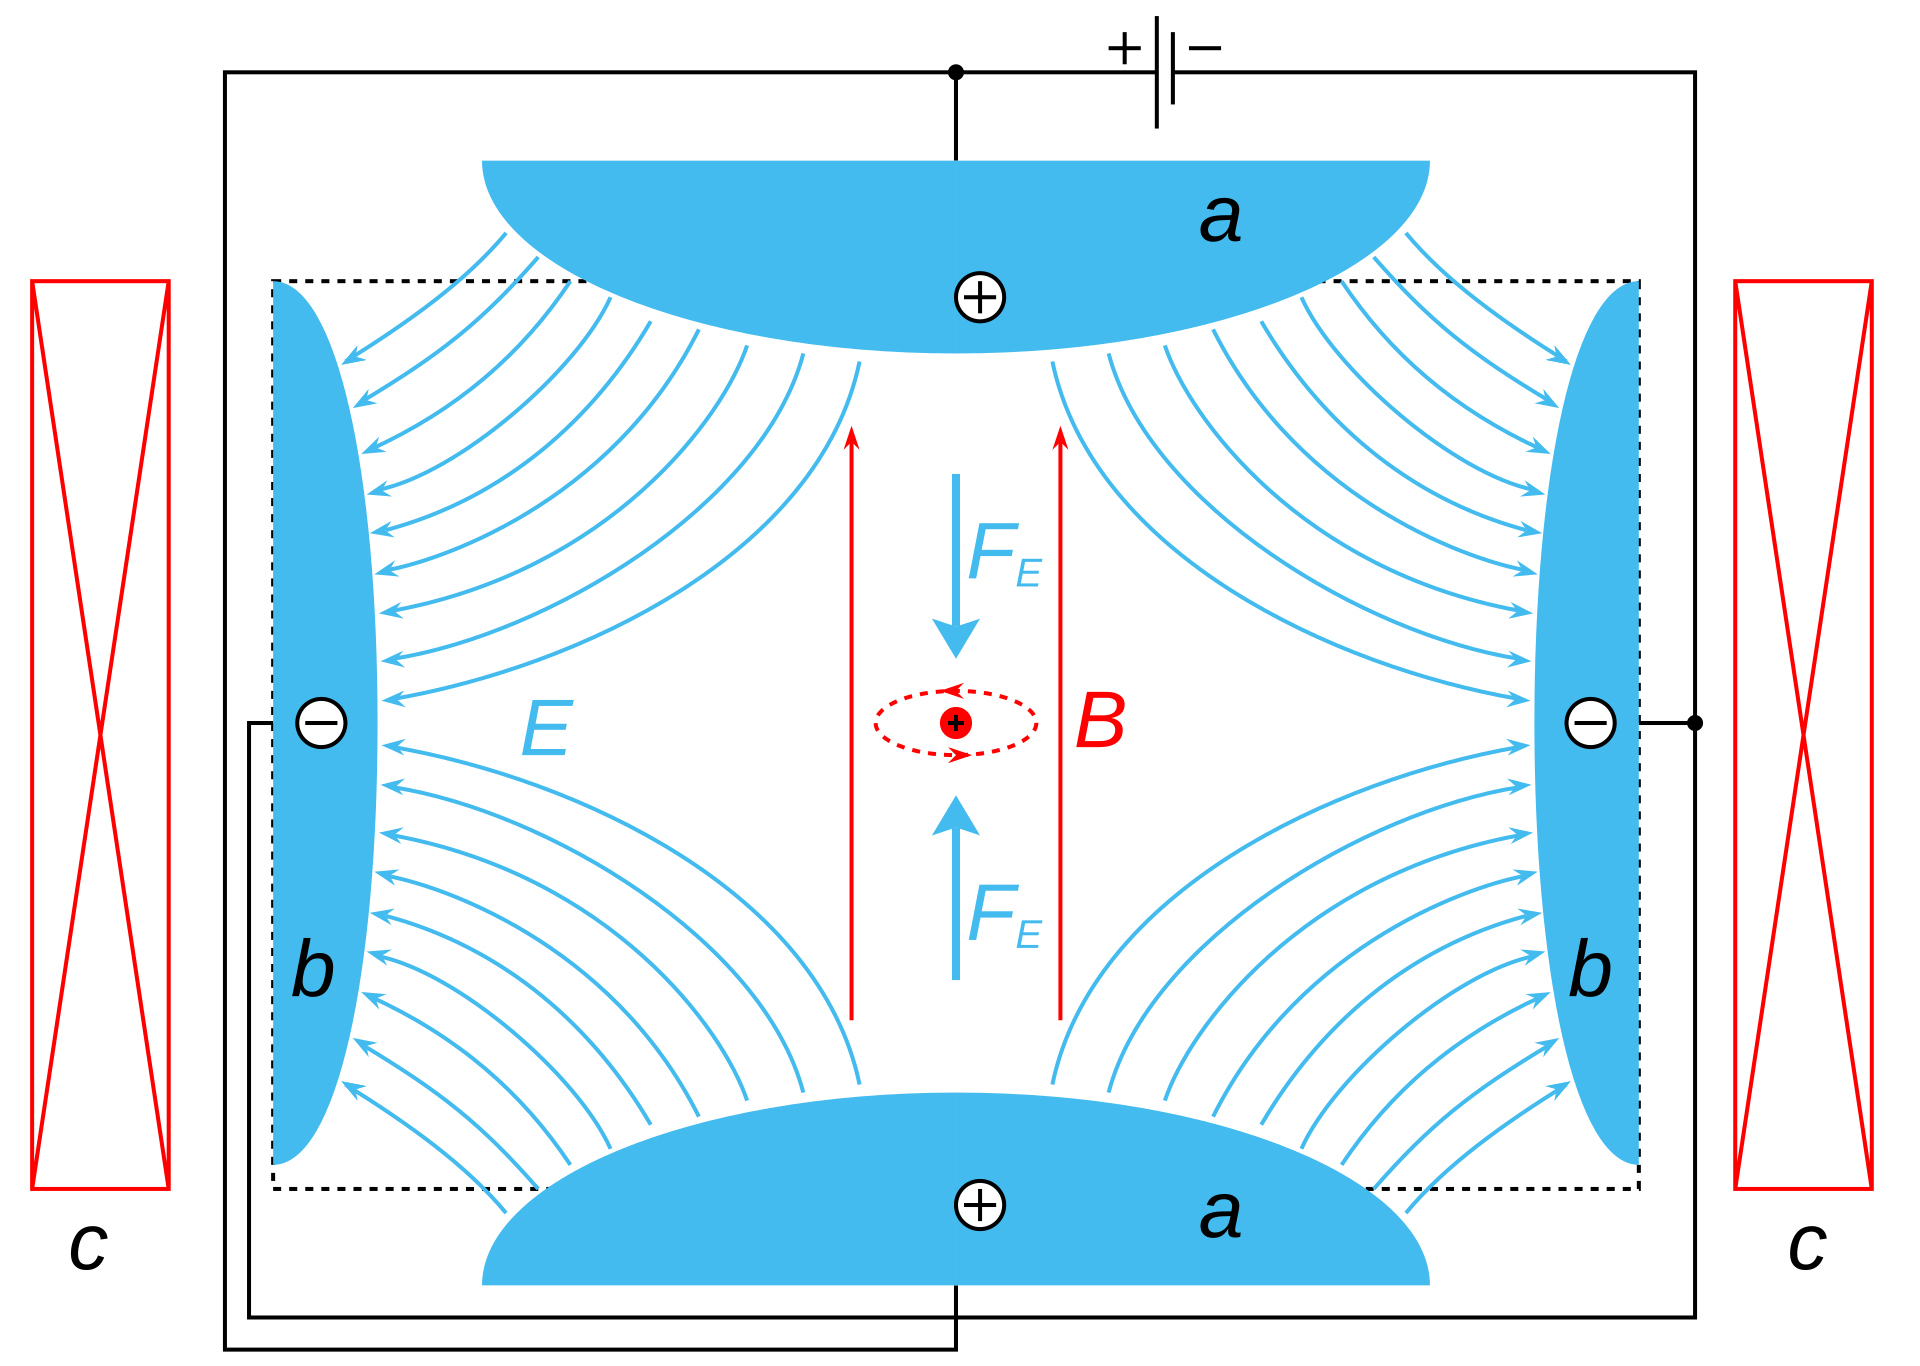
\includegraphics[width = 0.5 \textwidth]{Figures/Penning_Trap.png}
    \caption{Schematic of a Penning trap, further details are provided in \cref{sec:penningtrap}. This illustration is by Arian Kriesch and taken from \url{Wikimedia Commons}}
    \label{fig:penningtrap}
\end{figure}
\Cref{fig:penningtrap} displays a basic schematic for a Penning trap. 
It consists of two positively charged end-cap electrodes (a) and a negatively charged ring electrode (b).
These electrodes generate a static quadrupole electric field (E). The resulting inward electric forces ($F_E$) confine the positively charged particle along the vertical axis. 
Furthermore, external cylindrical magnets (c) produce a strong, uniform magnetic field pointing upwards in the $z$ direction. This field prevents escape by forcing the particle into a continuous orbital trajectory (dashed red path) in the horizontal plane. \cite{PenningTrapbook}\\
The force applied to the particles inside the trap is the Lorentz Force \cite{LectureNotes}:
\begin{align*} \bold{F} = q\bold{E} + q (\bold{v} \times \bold{B}), \end{align*}
In general, the electric field is given as
\begin{align*} \bold{E} = -\nabla(V), \end{align*}
with the potential of the Penning trap \cite{PenningTrapbook}
\begin{align*} V(x,y,z) = \frac{V_0}{2d^2} \cdot (2z^2 -x^2- y^2) \, \text{with} \, d \, = \, \sqrt{z_0^2 + \frac{r_0^2}{2}}, \end{align*}
where $z_0$ is the distance from the centre to the end caps and $r_0$ is the distance from the centre to the ring.)
The electric field is therefore given by:
\begin{align*}
    E_x &= -\frac{\partial}{\partial x}(\frac{V_0}{2d^2} (2z^2 -x^2-y^2) = \frac{V_0}{d^2} \cdot x, \\
    E_y &= -\frac{\partial}{\partial y}(\frac{V_0}{2d^2} (2z^2 -x^2-y^2) = \frac{V_0}{d^2} \cdot y, \\
    E_z &= -\frac{\partial}{\partial z}(\frac{V_0}{2d^2} (2z^2 -x^2-y^2) = \frac{-2V_0}{d^2} \cdot z.
\end{align*}
As the Lorentz Force is the only force acting upon the particle, Newton's second law for one particle with charge $q$ can be written as:
\begin{itemize}
    \item $\mathbf{x-direction}$:
    \begin{align}\label{eq:xdirect}
        m\ddot{x} &= qE_x + q(\mathbf{v} \times \mathbf{B})_x \notag \\
        m\ddot{x} &= qE_x + q\dot{y}B_0 \notag \\
        m\ddot{x} &= q\frac{V_0}{d^2}x + q\dot{y}B_0 \notag \\
        \Leftrightarrow 0 &= \ddot{x} - \frac{qV_0}{md^2}x - \frac{qB_0}{m}\dot{y} = \ddot{x} - \frac{1}{2}\omega_z^2 x - \omega_0 \dot{y}.
    \end{align}

    \item $\mathbf{y-direction}$:
    \begin{align}\label{eq:ydirect}
        m\ddot{y} &= qE_y - q\dot{x}B_0 \notag \\
        m\ddot{y} &= q\frac{V_0}{d^2}y - q\dot{x}B_0 \notag \\
        \Leftrightarrow 0 &= \ddot{y} - \frac{qV_0}{md^2}y + \frac{qB_0}{m}\dot{x} = \ddot{y} - \frac{1}{2}\omega_z^2 y + \omega_0 \dot{x}.
    \end{align}

    \item $\mathbf{z-direction}$:
    \begin{align}\label{eq:zdirect}
        m\ddot{z} &= qE_z + 0 \notag \\
        \Leftrightarrow 0 &= \ddot{z} + \frac{2qV_0}{md^2}z \notag \\
        0 &= \ddot{z} + \omega_z^2 z.
    \end{align}
\end{itemize}
For simplicity, we define $\omega_z^2 = \frac{2qV_0}{md^2}$ and $\omega_0 = \frac{qB_0}{m}$.
The solution for the z-direction is well-known as it is a harmonic oscillator with the general solution:
\begin{align} \label{eq: zana} z = A \cdot \cos{\omega_z t} + B \cdot \sin{\omega_z t}. \end{align}
Here, the constants $A$ and $B$ have to be calculated from the given initial conditions for the respective particle.
Our simulations will include both the starting position $\bold{r}$ and the starting velocity $\bold{v}$ as initial conditions.
From these, we can calculate the two constants using the z-components of the respective vectors by substituting $t=0$ into \cref{eq: zana}.
\begin{equation*}
    z(t=0) = A,
\end{equation*}
\begin{equation*}
    \frac{dz(t=0)}{dt} = B \omega_z.
\end{equation*}
To solve the DEs for the other directions we introduce a new complex-valued function $f(t) = x(t) + iy(t)$, with the first and second derivative $\dot{f(t)} = \dot{x(t)} + i\dot{y(t)}$ and $\ddot{f(t)} = \ddot{x(t)} + i\ddot{y(t)}$.
Adding \cref{eq:xdirect} and $i$ times \cref{eq:ydirect}, we find the following form:
\begin{align*} \ddot{x} + i\ddot{y} + \omega_0(i\dot{x} - \dot{y}) -\frac{1}{2}\omega_z^2 (x + iy) = 0. \end{align*}
This can be associated with the introduced function $f(t)$, the final form is then:
\begin{align}\label{eq:finalform} \ddot{f{t}} + i\omega_0 \dot{f(t)} - \frac{1}{2} \omega_z^2 f(t) = 0. \end{align}
To solve \cref{eq:finalform}, we choose a complex ansatz of the form
\begin{equation} \label{eq:Analyticalxy}
    f(t) = A_+ e^{-i(\omega_+ t + \phi_+)} + A_- e^{-i(\omega_- t + \phi_-)},  
\end{equation}
where $\phi_+$ and $\phi_-$ are constant phases, the amplitudes $A_+$ and $A_-$ are positive, and
\begin{align}\label{eq:omegapm}\omega_\pm = \frac{\omega_0 \pm \sqrt{\omega_0^2 - 2\omega_z^2}}{2}.\end{align}
The two rotary motions, whose superposition make up this analytical solution in the x and y coordinates, are usually called the magnetron drift ($\omega_-$ rotation) and the cyclotron motion ($\omega_+$ rotation)\cite{PenningTrapbook}.
The physical coordinates are found as $x(t) = \text{Re} (f(t))$ and $y(t) = \text{Im} (f(t))$.
To find a realistic solution, we have to pay attention to the following restriction: 
The solution of $f(t)$ should remain bounded even for high values for $t$ ($|f(t)| < \infty \text{ for } t \rightarrow \infty$).
The constraint on $\omega_{\pm}$ for containment is that it has to be a real number. Elsewhere, the exponent will not be complex anymore for one summand (because we could write then $\omega_{\pm}$ as a complex number of the form $a+ib$ and as $i \cdot i$ is real one exponent looks like $e^{bt}$). To avoid this, the square root in \cref{eq:omegapm} has to be positive. Thus, $$\omega_0^2 > 2\omega_z^2$$ has to hold \cite{PenningTrapbook}. Written in terms of the constants given by the Penning trap configuration, this leads to \cref{eq:stability}.
\begin{equation} \label{eq:stability}
    \frac{q}{m} > \frac{4V_0}{d^2B_0^2}.
\end{equation}
To calculate the distance from the particle to the origin inside the x-y plane, we will use the triangle inequality to approximate the maximum as well as the minimum value. For every time, we know:
$$R(t) = |f(t)| = |A_+ e^{-i(\omega_+ t + \phi_+)} + A_- e^{-i(\omega_- t + \phi_-)}|.$$
For the upper bound, we use the triangle inequality:
\begin{align*}
R(t) &\le |A_+ e^{-i(\omega_+ t + \phi_+)}| + |A_- e^{-i(\omega_- t + \phi_-)}| \\
&= |A_+| + |A_-| = A_+ + A_- = R_+.
\end{align*}
For the lower bound, we use the reverse triangle inequality:
\begin{align*} 
R(t) &\ge ||A_+ e^{-i(\omega_+ t + \phi_+)}| - |A_- e^{-i(\omega_- t + \phi_-)}|| \\
&= ||A_+| - |A_-|| = |A_+ - A_-| = R_-. \end{align*}
For further tests in \cref{sec:results_and_discussion}, we need to introduce initial conditions in order to find a specific analytic solution. In our first investigation, using only a single particle, these are given by:
\begin{align}
    \centering
    x(0) &= x_0 > 0 &\text{ and } \dot{x}(0) &= 0, \\
    y(0) &= 0 &\text{ and } \dot{y}(0) &= v_0 > 0, \\
    z(0) &= z_0 &\text{ and } \dot{z}(0) &= 0.
\end{align}
Thus (see \cref{eq:zdirect}):
\begin{align*}
    z(t) = z_0 \cos{\omega_zt}.
\end{align*}
Considering a movement in the $xy$-plane, a specific solution is given by \cref{eq:finalform} with:
\begin{align*}
    A_+ &= \frac{v_0 + \omega_- x_0}{\omega_+ - \omega_-}\footnotemark, & A_- &= \frac{v_0 + \omega_+ x_0}{\omega_+ - \omega_-}, \\[10pt]
    \phi_+ &= \pi, & \phi_- &= 0.
\end{align*}
\footnotetext{For general initial conditions, the amplitudes and the phases are moduli and negative arguments of complex numbers.}
For $n$ particles with charges $\{q_1, ... , q_n\}$ and masses $\{m_1, ... , m_n\}$ the differential equations have the following form:
\begin{align*}
    \ddot{x}_i - \omega_{0,i} \dot{y}_i - \frac{1}{2} \omega_{z,i}^2 x_i - k_e \frac{q_i}{m_i} \sum_{j \neq i} q_j \frac{x_i - x_j}{|\mathbf{r}_i - \mathbf{r}_j|^3} &= 0, \\[10pt]
    \ddot{y}_i + \omega_{0,i} \dot{x}_i - \frac{1}{2} \omega_{z,i}^2 y_i - k_e \frac{q_i}{m_i} \sum_{j \neq i} q_j \frac{y_i - y_j}{|\mathbf{r}_i - \mathbf{r}_j|^3} &= 0, \\[10pt]
    \ddot{z}_i + \omega_{z,i}^2 z_i - k_e \frac{q_i}{m_i} \sum_{j \neq i} q_j \frac{z_i - z_j}{|\mathbf{r}_i - \mathbf{r}_j|^3} &= 0.
\end{align*}
The Coulomb force couples the equations for two or more particles, leading to non-linear dynamics, which are generally difficult to solve analytically. 
Instead, researchers have relied on numerical methods to study this system, as was done in e.g. \cite{NumericalPenning1}.
Here, we introduce numerical approaches such as RK4 and FE to treat this coupled system of equations. 
However, both of them are expecting a first-order DE. The associated first-order DEs are:
\begin{align} \label{eq: coupledstart}
    \centering
    \dot{x}_i &= v_{x,i}, \\
    \dot{y}_i &= v_{y,i}, \\
    \dot{z}_i &= v_{z,i}, \\
    \dot{v}_{x,i} &= \omega_{0,i} v_{y,i} + \frac{1}{2} \omega_{z,i}^2 x_i + k_e \frac{q_i}{m_i} \sum_{j \neq i} q_j \frac{x_i - x_j}{|\mathbf{r}_i - \mathbf{r}_j|^3}, \label{eq:vstart} \\[8pt] 
    \dot{v}_{y,i} &= -\omega_{0,i} v_{x,i} + \frac{1}{2} \omega_{z,i}^2 y_i + k_e \frac{q_i}{m_i} \sum_{j \neq i} q_j \frac{y_i - y_j}{|\mathbf{r}_i - \mathbf{r}_j|^3}, \\[8pt]
    \dot{v}_{z,i} &= -\omega_{z,i}^2 z_i + k_e \frac{q_i}{m_i} \sum_{j \neq i} q_j \frac{z_i - z_j}{|\mathbf{r}_i - \mathbf{r}_j|^3}. \label{eq: coupledend}
\end{align}
Unless indicated otherwise, our simulation results and the associated code use the following configurations:
\begin{equation*}
    B_0 = 1.00\,\mathrm{T} \simeq 9.65 \times 10^1 \, \frac{\mathrm{u}}{(\mathrm{\mu s}) \, \mathrm{e}},
\end{equation*}
\begin{equation*}
    V_0 = 25.0\,\mathrm{mV} \simeq 2.41 \times 10^6 \, \frac{\mathrm{u} \, (\mathrm{\mu m})^2}{(\mathrm{\mu s})^2 \, \mathrm{e}},
\end{equation*}
\begin{equation*}
    d = 500\,\mathrm{\mu m}.
\end{equation*}
The particles we simulate are singly-charged \(\ce{^{40}Ca}\) ions. We chose to use this particular isotope, as it is the most abundant naturally occurring \(\ce{Ca}\) isotope. \cite{CAWeight} Therefore the weight of the particles will be: $m = 39.962 590 863 u$.
Given these constants, we can predict if the constructed Penning trap can contain a single \(\ce{^{40}Ca}\) ion stably by using \cref{eq:stability}.
\begin{equation*}
    \frac{1 e}{39.962 590 863 u} > \frac{4 \cdot 2.41 \cdot 10^6 \, \frac{\mathrm{u} \, (\mathrm{\mu m})^2}{(\mathrm{\mu s})^2 \, \mathrm{e}}}{\left (500 \mu m \cdot 9.65 \times 10^1 \, \frac{\mathrm{u}}{(\mathrm{\mu s}) \, \mathrm{e}} \right)^2}
\end{equation*}
\begin{equation*}
    0.0250234026 > 4.140782303 \cdot 10^{-3}
\end{equation*}
Therefore, we expect our simulation to show that a single particle stays contained inside the trap.

\subsection*{Numerical algorithms}\label{sec:Algorithms}

We use both FE and RK4 to solve the differential equations derived in the above section.
FE is used as a point of comparison for RK4, as the implementation of the more accurate RK4 method can be complicated for coupled differential equations.

\subsubsection{Forward Euler}
The FE method is one of the simplest algorithms to numerically approximate the solution to ordinary differential equations. For a non-coupled differential equation, it can be written as \cite{Faul2016ACI}:
\begin{equation*}
    y_{i+1} = y_i + dt \cdot f(t_i,y_i)
\end{equation*}
As our equations (\cref{eq: coupledstart}-\cref{eq: coupledend}), which describe the movements of particles inside a Penning trap, are coupled, the method has to be rewritten into the form of \cref{eq:FEv} and \cref{eq:FEx}. Furthermore, we have to keep in mind that the equations describing our particles are three-dimensional and we therefore need to use vectors to describe the motion of the particles\cite{LectureNotes}. 
\begin{equation}\label{eq:FEv}
    \boldsymbol{v}_{i+1} = \boldsymbol{v}_i + dt \cdot f(t_i, \boldsymbol{r}_i, \boldsymbol{v}_i)
\end{equation}
\begin{equation}\label{eq:FEx}
    \boldsymbol{r}_{i+1} = \boldsymbol{r}_i + dt \boldsymbol{v}_i
\end{equation}
For an initial value problem similar to the one posed through the coupled differential equations of the Penning trap, the local error of FE is $\mathcal{O}(dt^2)$. 
Therefore, the global error of this method is of order $\mathcal{O}(dt)$.

\subsubsection{Runge-Kutta-4}
Similar to FE, RK4 is a numerical method for solving first-order differential equations of the form:
\begin{equation*}
    \frac{dy}{dt} = f(t,y).
\end{equation*}
The Butcher tableau for RK4 is given by \cref{tab:RK4-Butcher} \cite{Faul2016ACI}.
\begin{table}[h]
    \centering
    \caption{Butcher Tableau for the RK4 method.}
    \begin{tabular}{c|cccc}
        0 & \\
        0.5 & 0.5\\
        0.5 & 0 & 0.5\\
        1 & 0 & 0 & 1 \\
        \hline
         & $\frac{1}{6}$ & $\frac{1}{3}$ & $\frac{1}{3}$ & $\frac{1}{6}$
    \end{tabular}
    \label{tab:RK4-Butcher}
\end{table}
Therefore, we can describe RK4 for non-coupled differential equations using the pseudo-code given in \cref{algo:RK4} \cite{LectureNotes}. 
\begin{figure}[H]
    \begin{algorithm}[H]\label{algo:RK4}
        \caption{RK4 Algorithm}
        \label{algo:RK4}

        \begin{algorithmic}[1]
           \Require Number of timesteps $N_t$,
                    step size $dt$,
                    function $f(t,y)$,
                    Initial condition(s): $y_0$, $t_0=0$

        \For{$i=0$; $i < N_t$; i++}

            \State $k_0 \gets dt f(t_i, y_i)$
            \State $k_2 \gets dt f(t_i+ 0.5 \cdot dt, y_i+ 0.5 k_1)$
            \State $k_3 \gets dt f(t_i+ 0.5 \cdot dt, y_i+ 0.5 k_2)$
            \State $k_4 \gets dt f(t_i + \cdot dt, y_i+ k_3)$

            \State $y_{i+1} = y_i + \frac{1}{6}(k_1 + 2k_2 + 2k_3 + k_4)$
            \State $t_i \gets t_i + dt$
         \EndFor

        \State \Return $y$
        \end{algorithmic}
    \end{algorithm}
\end{figure}
This algorithm has a local error of order $\mathcal{O}(dt^5)$, which equates to a global error of order $\mathcal{O}(dt^4)$.
For coupled differential equations, this algorithm has to be changed, as the calculation of the different $k$'s for every equation requires the approximated intermediate points of the other equations.
\begin{figure}[h]
    \begin{algorithm}[H]
        \caption{RK4 algorithm for coupled differential equations}
        \label{algo:RK4couple}

        \begin{algorithmic}[1]
            \Require Number of time steps $N_t$, step size $dt$,
                     function $\boldsymbol{f}(t,\boldsymbol{x},\boldsymbol{v})$,
                     initial conditions $\boldsymbol{x}_0$, $\boldsymbol{v}_0$,
                     and $t_0=0$

            \For{$i = 0$ to $N_t-1$}
                \State $\boldsymbol{k}_{\boldsymbol{x},1} \gets dt\boldsymbol{v}_i$
                \State $\boldsymbol{k}_{\boldsymbol{v},1} \gets
                    dt\boldsymbol{f}(t_i,\boldsymbol{x}_i,\boldsymbol{v}_i)$ 
                \Statex %Empty line
                \State $\boldsymbol{k}_{\boldsymbol{x},2} \gets
                    dt\left(\boldsymbol{v}_i+\frac{1}{2}k_{\boldsymbol{v},1}\right)$
                \State $\boldsymbol{k}_{\boldsymbol{v},2} \gets
                    dt\boldsymbol{f}\left(
                    t_i+\frac{1}{2}dt,\,
                    \boldsymbol{x}_i+\frac{1}{2}k_{\boldsymbol{x},1},\,
                    \boldsymbol{v}_i+\frac{1}{2}k_{\boldsymbol{v},1}
                    \right)$ 
                \Statex %Empty line
                \State $\boldsymbol{k}_{\boldsymbol{x},3} \gets
                    dt\left(\boldsymbol{v}_i+\frac{1}{2}k_{\boldsymbol{v},2}\right)$
                \State $\boldsymbol{k}_{\boldsymbol{v},3} \gets
                    dt\boldsymbol{f}\left(
                    t_i+\frac{1}{2}dt,\,
                    \boldsymbol{x}_i+\frac{1}{2}k_{\boldsymbol{x},2},\,
                    \boldsymbol{v}_i+\frac{1}{2}k_{\boldsymbol{v},2}
                    \right)$ 
                \Statex %Empty line
                \State $\boldsymbol{k}_{\boldsymbol{x},4} \gets
                    dt\left(\boldsymbol{v}_i+k_{\boldsymbol{v},3}\right)$
                \State $\boldsymbol{k}_{\boldsymbol{v},4} \gets
                    dt\boldsymbol{f}\left(
                    t_i+dt,\,
                    \boldsymbol{x}_i+k_{\boldsymbol{x},3},\,
                    \boldsymbol{v}_i+k_{\boldsymbol{v},3}
                    \right)$ 
                \Statex %Empty line
                \State $\boldsymbol{x}_{i+1} \gets \boldsymbol{x}_i
                    +\frac{1}{6}\left(
                    \boldsymbol{k}_{\boldsymbol{x},1}+2\boldsymbol{k}_{\boldsymbol{x},2}
                    +2\boldsymbol{k}_{\boldsymbol{x},3}+\boldsymbol{k}_{\boldsymbol{x},4}
                    \right)$ 
                \State $\boldsymbol{v}_{i+1} \gets \boldsymbol{v}_i
                    +\frac{1}{6}\left(
                    \boldsymbol{k}_{\boldsymbol{v},1}+2\boldsymbol{k}_{\boldsymbol{v},2}
                    +2\boldsymbol{k}_{\boldsymbol{v},3}+\boldsymbol{k}_{\boldsymbol{v},4}
                    \right)$ 
                \State $t_{i+1} \gets t_i+dt$
            \EndFor

            \State \Return $\boldsymbol{x},\boldsymbol{v}$
        \end{algorithmic}
    \end{algorithm}
\end{figure}

For our implementations of the numerical solver for equations \ref{eq: coupledstart} - \ref{eq: coupledend}, we rewrote this algorithm to the form presented in \cref{algo:RK4couple}. This also required us to reformulate all variables of the problem into vectors, as the set of equations \ref{eq: coupledstart} - \ref{eq: coupledend} presents a 3-dimensional problem.

In the implementation $\boldsymbol{f}(t,\boldsymbol{x},\boldsymbol{v})$ forms the right hand side of \cref{eq:vstart} - \cref{eq: coupledend}. If there is more than one particle in the Penning trap, the algorithm has to calculate all values $k_i$ for every particle before calculating the next $k_{i+1}$ and before taking a step. This is caused by the coupling between particles introduced through the Coulomb force in \cref{eq:vstart} - \cref{eq: coupledend}. \\
In our code, both FE and RK4 are implemented as classes, which are passed to a Penning trap and evolve the system for a given time step.

One of our goals is to compare the accuracy of both methods and the convergence towards the analytical solution. Therefore, we conduct a numerical study with $n_1 =4000, \, n_2 = 8000, \, n_3 =16000$ and $n_4=32000$ time steps for a single particle Penning trap, which are then compared to the analytical solutions derived above.

For Hamiltonian systems, symplectic methods conserve the phase space volume of the system and can therefore create a bound on the energy error. However, neither FE nor RK4 is a symplectic method. Therefore, we do not expect the implemented methods to conserve the phase space volume of our system, which can result in a drift in total energy, even if our analytical prediction is for a system to stay stable. \cite{LectureNotes}

\subsection*{Tools}

We used the Python library \texttt{matplotlib} \cite{Hunter:2007} to produce all illustrations in this report. The underlying C++ Code depends on the library \texttt{Armadillo} \cite{sanderson2025armadillo}. Large language models GPT 6-Luna and Gemini 4-Argon were used in order to debug small parts of the produced code.
% ===========================================
\section{Results and discussion}\label{sec:results_and_discussion}
\subsubsection*{One Particle simulation}\label{sec:OnePart}

We conducted a simulation of a single particle using both the FE and the RK4 method to evolve the Penning trap over a total time frame of $50 \mu s$. 
For the setup of the trap, we used the conditions outlined in \cref{sec:penningtrap}, while initialising the particle at the position $\bold{r}=(20, 0, 20) \mu m$ with the velocity $\bold{v} = (0, 25, 0)\mu m/\mu s$.
\begin{figure}[h]
    \centering
    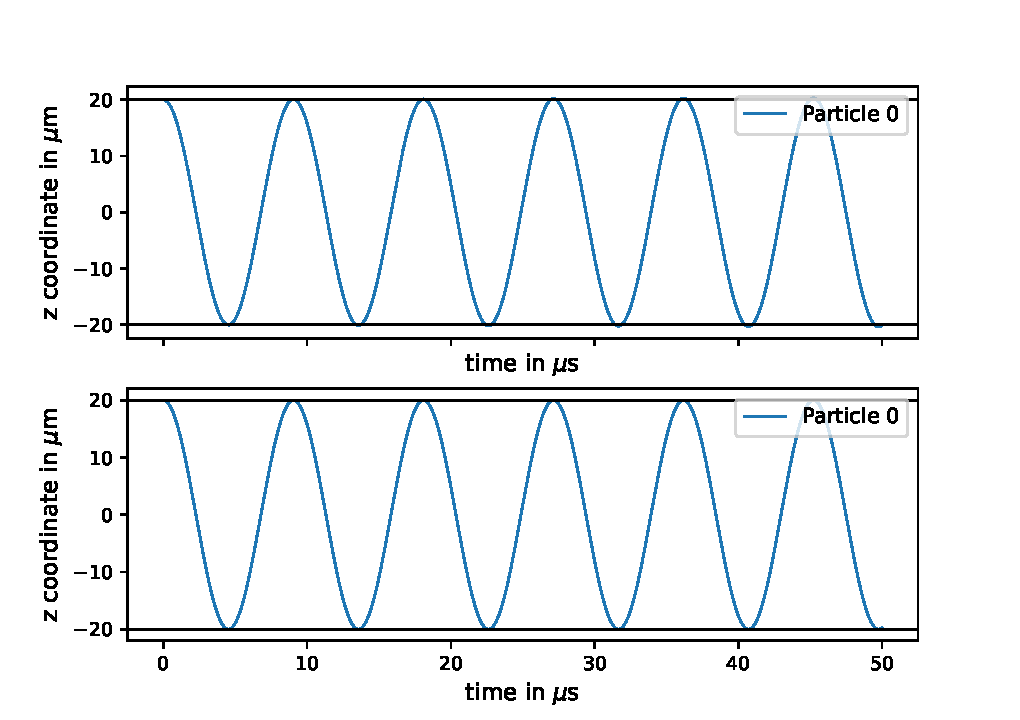
\includegraphics[width = 0.45 \textwidth]{Figures/RK4_vs_FE_z-t-plot.pdf}
    \caption{Evolution of the z-coordinate of a single particle over 50 $\mu s$. The upper plot shows the simulation using FE with 32000 time steps, the lower plot shows the simulation using RK4 with 32000 time steps.}
    \label{fig:z-t-singleparticle}
\end{figure}

\begin{figure}[h]
    \centering
    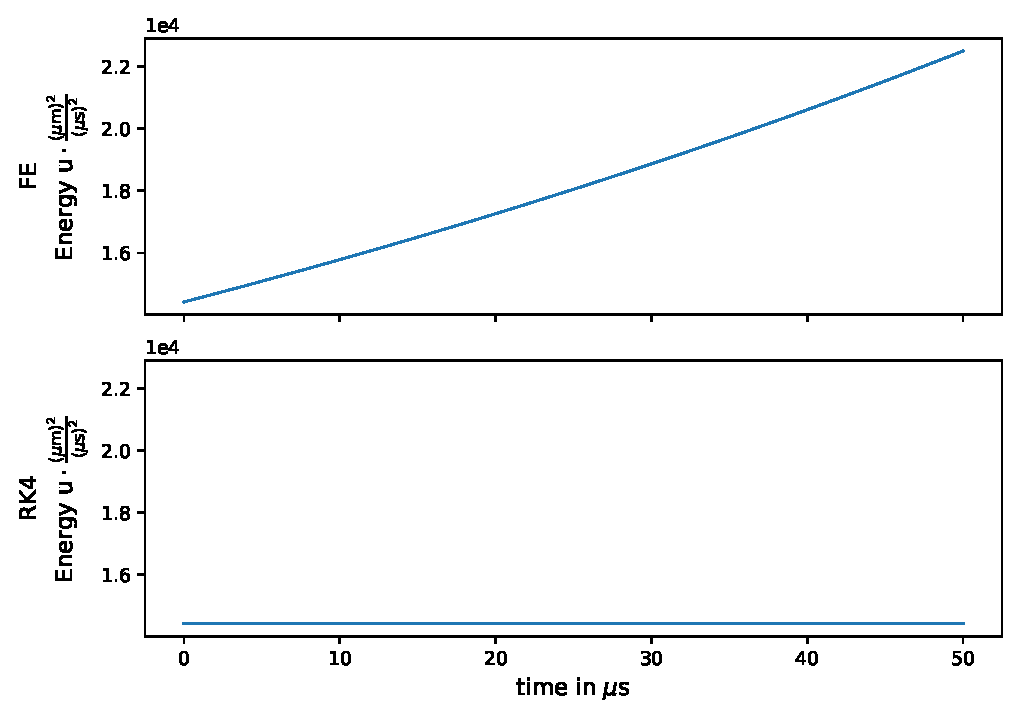
\includegraphics[width = 0.45 \textwidth]{Figures/RK4_vs_FE_total_energy.pdf}
    \caption{Total energy of the particle as a function of time. The upper plot shows the total energy in the FE simulation with 32000 time steps, the lower plot shows the total energy in the RK4 simulation with 32000 time steps.}
    \label{fig:energy}
\end{figure}

\Cref{fig:z-t-singleparticle} shows the particle's z-coordinate over the simulated time frame of $50 \mu s$ using both the FE (upper figure) and RK4 method (lower figure).
The vertical black lines show our expected upper and lower bounds for the particle's z position, as we expect this particle to move according to \cref{eq: zana}.
However, as discussed previously, neither FE nor RK4 is a symplectic method, and we do not expect them to accurately conserve energy.
When viewing the z-t-plot in the FE plot, this behaviour becomes obvious, as the simulated particle violates the theoretical maximum and minimum bounds of the z-coordinate. 
\footnote{This also becomes obvious when viewing an animation in the x-y-plane, where the circular motion in FE shows larger and larger circles. Such animations are saved under the  {\href{https://github.uio.no/johascha/CompPhys/tree/804b9bde4149b083d3da74c53a158c031194d2bb/Project_3/figures/Animations}{Animations folder}}.}

The failure of not conserving energy is also shown in \Cref{fig:energy}, where the total energy of the particle is displayed for both the FE and the RK4 method. 
We calculated this total energy as the sum of the kinetic energy of the particle and the potential energy given through the electric field and the charge of the ion.
The upper plot, which displays the energy of the particle in the FE, shows a near-constant energy drift. 
This causes the deviation from the analytical solution and would also be the cause for the simulated particle to not stay contained on a larger time scale, even though it is predicted to do so by the stability condition derived previously in section \cref{sec:penningtrap}.
In contrast, the more accurate RK4 method does not violate the bound in \Cref{fig:z-t-singleparticle}, as the method, in this case, is sufficiently more accurate to approach the real solution even after 50 $\mu s$. 
Furthermore, RK4 also does not show a significant energy drift in \Cref{fig:energy}, which is in line with what is seen in \Cref{fig:z-t-singleparticle}. 
Note that even though there is no significant energy drift observed in the simulation, RK4 can still cause drifts in the total energy. 
This was merely not observed here, because of the higher level of accuracy in comparison to FE and the high number of discretization points (32000).\\
In order to quantify the relative error of the calculations, our single particle simulation was compared to the analytical solution derived in \ref{sec:methods}.
To assess the accuracy, we defined the relative error as:
\begin{equation*}
    \epsilon_i = \frac{|\mathbf{r}_{i, \text{exact}} - \mathbf{r}_i|}{|\mathbf{r}_{i, \text{exact}}|}.
\end{equation*}

\begin{figure}[H]
    \centering
    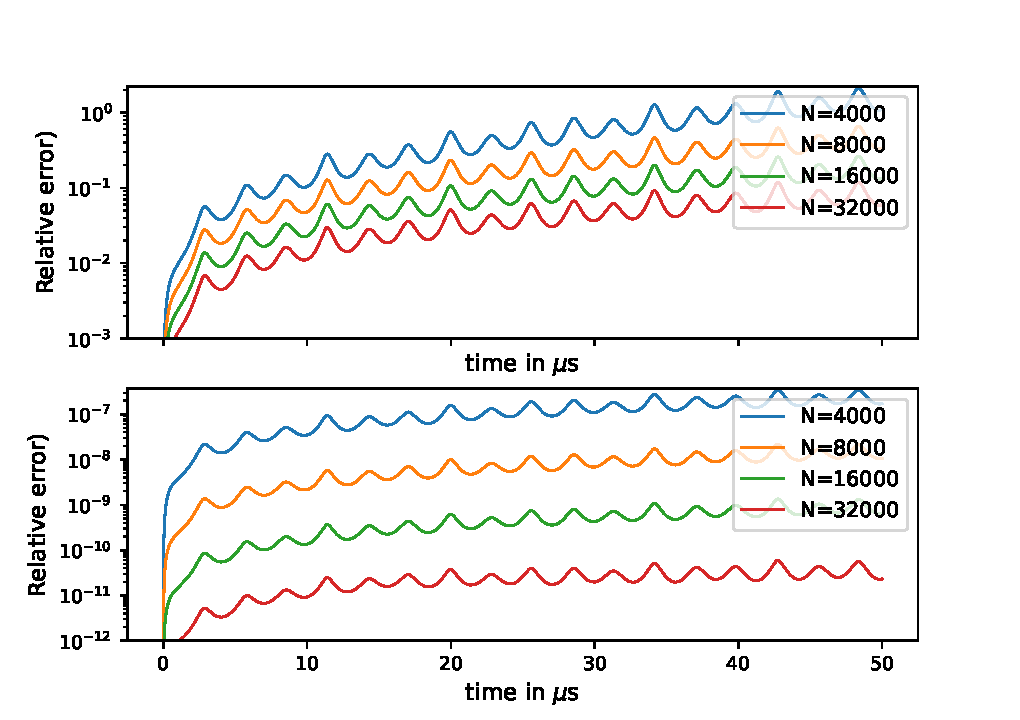
\includegraphics[width = 0.45 \textwidth]{Figures/RK4_vs_FE_rel_error-plot.pdf}
    \caption{Evolution of the relative error between the analytical and the numerical solution using FE (upper figure) and RK4 (lower figure). The differently coloured lines indicate different discretisation levels.}
    \label{fig:rel_error}
\end{figure}
The numerical superiority of RK4 can also be seen in \Cref{fig:rel_error}, where the relative error to the analytical solution is compared for different amounts of discretisation points.
To make the graphs more readable, the FE plot is cut off at a minimum relative error of $10^{-3}$, while the RK4 plot is cut off at a value of $10^{-12}$, with the y-axis being logarithmically scaled in both graphs.
As noted in \cref{sec:methods}, the FE has a global error of order $\mathcal{O}(dt)$, while the global error of RK4 is of order $\mathcal{O}(dt^4)$.

\begin{table}[ht]
    \centering
    \caption{Final relative errors for Forward Euler and RK4 methods.}
    \label{tab:error-comparison}
    \begin{tabular}{ccccc}
        \hline
        $\Delta t$ ($\mu\mathrm{s}$) &
        $\epsilon_{\mathrm{FE}}$ &
        $\epsilon_{\mathrm{RK4}}$ &
        $\epsilon_{\mathrm{FE}} / \Delta t$ &
        $\epsilon_{\mathrm{RK4}} / (\Delta t)^4$ \\
        \hline
        $1.25 \times 10^{-2}$ & $1.10$ & $1.70 \times 10^{-7}$ & $87.86$ & $6.98$ \\
        $6.25 \times 10^{-3}$ & $0.33$ & $1.07 \times 10^{-8}$ & $53.45$ & $6.98$ \\
        $3.13 \times 10^{-3}$ & $0.13$ & $6.58 \times 10^{-10}$ & $42.61$ & $6.90$ \\
        $1.56 \times 10^{-3}$ & $0.06$ & $2.31 \times 10^{-11}$ & $38.26$ & $3.88$ \\
        \hline
    \end{tabular}
\end{table}
\Cref{tab:error-comparison} shows the final relative errors for both FE and RK4 for all selected numbers of time steps.
The last two columns show the ratio between the final relative error and the step size to the power of the expected order of convergence for the two methods (1 for the FE method and 4 for the RK method).
These values are of interest, as the ratio between the final error and the suspected convergence order can approximately determine the order of convergence.
As the values of both of the last two columns stay approximately constant in magnitude, our expectations for the error of the FE method to be of order $\mathcal{O}(dt)$ and for the error of the RK4 method to be of order $\mathcal{O}(dt^4)$ are roughly confirmed.
It is of note that, especially for the FE method, the errors show slightly better convergence than expected.
However, as this convergence measure was only done at a single point, cancellation there may affect the observed order, leading to strongly suggestive rather than conclusive results.

\subsubsection*{Two Particle simulation}\label{sec:OnePart}

\Cref{fig:2-particle-nointer} shows the paths of two particles inside the Penning trap simulated using the RK4 algorithm with no interactions.
Particle 0 has the same initial conditions as the particle in the single particle simulation, while particle 1 is initialised at the position $\bold{r}=(25, 25, 0) \mu m$ with the velocity $\bold{v} = (0, 40, 5)\mu m/\mu s$.

\begin{figure}[ht]
    \centering
    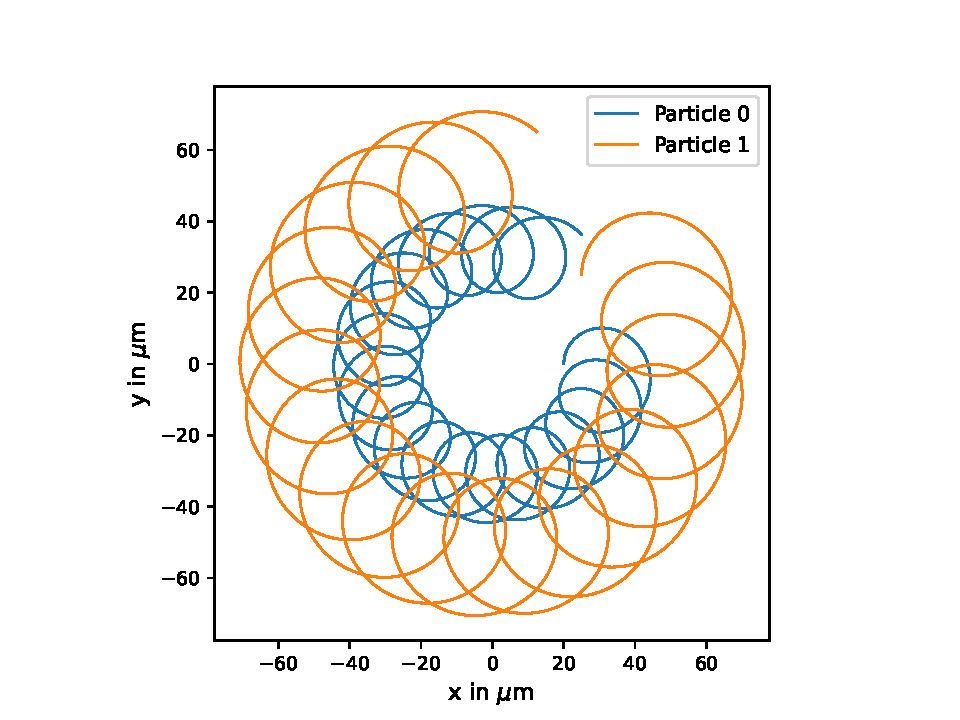
\includegraphics[width = 0.45 \textwidth]{Figures/RK_x_y_no_inter.pdf}
    \caption{The x-y-plane of two non-interacting particles inside the simulated Penning trap.}
    \label{fig:2-particle-nointer}
\end{figure}
As the underlying forces acting upon the particles have not changed in the case of no interaction, a similar picture as before arises.
Both particles perform two simultaneous orbital motions, comprised of a large orbit around the middle of the Penning trap, which is the magnetron drift, and a smaller, faster orbit, which is the cyclotron motion. 
This is in line with the analytical solution for single particles, which we found to be described by \cref{eq:Analyticalxy}, which features a superposition of two cylindrical motions.
In contrast, \Cref{fig:2-particle} shows the paths taken by two ions interacting through the Coulomb force, with the same initial conditions.
\begin{figure}[ht]
    \centering
    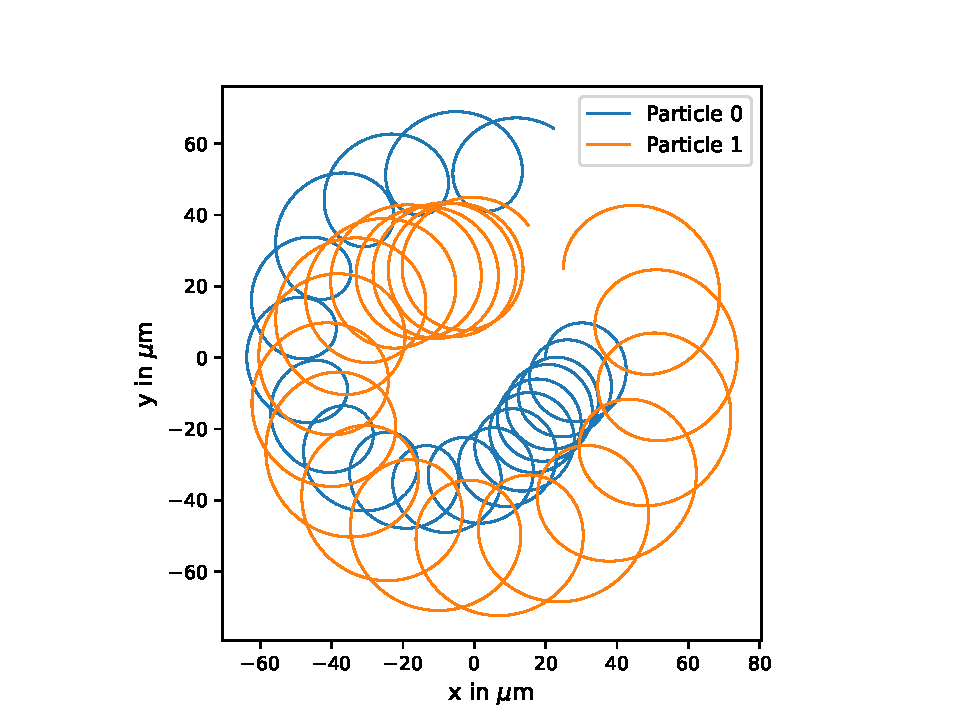
\includegraphics[width = 0.45 \textwidth]{Figures/RK_x_y.pdf}
    \caption{The x-y-plane of two particles interacting through the Coulomb force inside the simulated Penning trap.}
    \label{fig:2-particle}
\end{figure}

This creates significantly changed results for both of the particles, as the paths of the two particles now no longer orbit independently of each other.
Instead, the larger orbits of the two particles now overlap with each other, while the smaller, more frequent orbital motion shows varying speeds in comparison to the angular velocity of the larger orbital motion.
Both of these alterations can be explained through the introduction of the Coulomb force into the system.
While Particle 0 starts out further in the negative x direction than Particle 1, it will be pushed further in said direction, as long as Particle 1 has a larger x-coordinate.
A similar phenomenon can be seen in the y-direction. Here, Particle 1 has a larger y value at the start, however, due to the larger initial velocity and the initial position of the particle being further away from the origin, the y-value quickly shrinks below that of Particle 0.
During the time Particle 1 has a lower y value, it pushes Particle 0 into the positive y direction until it eventually reaches a higher y value towards the end of the simulation.
The transfer of energy through the Coulomb force couples the motion of the two particles, leading to a change in the angular velocity of both the cyclotron motion and the magnetron drift.
This therefore also explains the changes in the relative angular frequency between the two rotatory nodes.\\
The influence of the interactions through the Coulomb force can also be seen when viewing phase-space plots of the simulations.
\Cref{fig:phase-space-plots} shows both the x-$v_x$ and the z-$v_z$ phase space with and without interactions.

\begin{figure}[H]
    \centering
    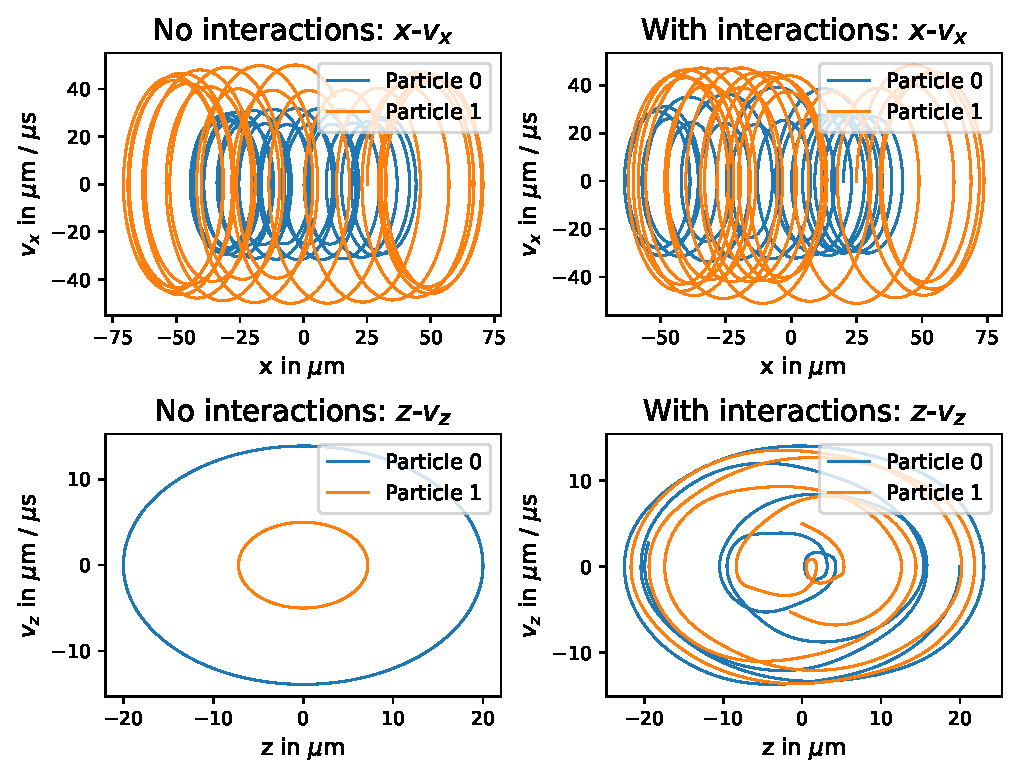
\includegraphics[width = 0.45 \textwidth]{Figures/RK4_two_particle_phase_space.pdf}
    \caption{The x-$v_x$ (upper row) and the z-$v_z$ (lower row) phase space in the RK4 simulation without (left column) and with interactions (right column).}
    \label{fig:phase-space-plots}
\end{figure}

While the z-$v_z$ phase space displays two stable oscillatory motions in the case of no interactions between the two particles, we can see clear coupling effects in the bottom right plot, which displays the z-$v_z$ phase space with interactions between the particles. 
This is in line with our expectation, as the repulsive Coulomb force transfers energy between the two particles, leading to continuous shifting in their phase space.
During this simulation of a 50 $\mu s$ time frame, both particles also remain bounded in the z-direction, as we previously had also seen in the x and y directions.


\subsubsection*{Perturbed Penning Traps}

The previously explored behaviour, although it brought great insight into how Penning traps work, was not entirely physical. That is because real-world experiments are not free of external perturbations, as was assumed. These perturbations can take various forms - for instance, the electromagnetic field can vary over time, potentially causing particles to escape the trap entirely. To investigate this possibility, we introduced a time-dependent term to the electric potential of our model:
\begin{equation}\label{eq:perturbation}
    V_0 \rightarrow V_0\left(1+f\cos(\omega_Vt)\right),
\end{equation}
where $f$ is a constant amplitude and $\omega_V$ is the angular frequency of the perturbation term.

Our subsequent analysis examined how the amplitude and angular frequency affect particle escape. The simulation setup consisted of 100 singly ionised Calcium-40 particles with randomised state vectors drawn from a normal distribution. The trap size and its magnetic field were kept as in previous tasks ($d=500$ $\mu\text{m}$, $B_0=1.00$ T), while the initial electric potential ($V_0=25.0$ mV) was perturbed according to eq. \ref{eq:perturbation}.

We then repeatedly simulated the evolution of the system for 500 $\mu$s with different values of $f$ and $\omega_V$, and counted how many particles were left inside the trap ($|\mathbf{r}|<d$). To get a coarse estimate of the resulting behaviour, we began with a broad sweep of angular frequencies ($\omega_V \in \left[0.2,2.5\right]$ MHz) with lower resolution to speed up computations ($d\omega = 0.02$ MHz). For each simulation, $40,000$ time steps were made, yielding $dt=0.0125$ $\mu$s. 

\begin{figure}
    \centering
    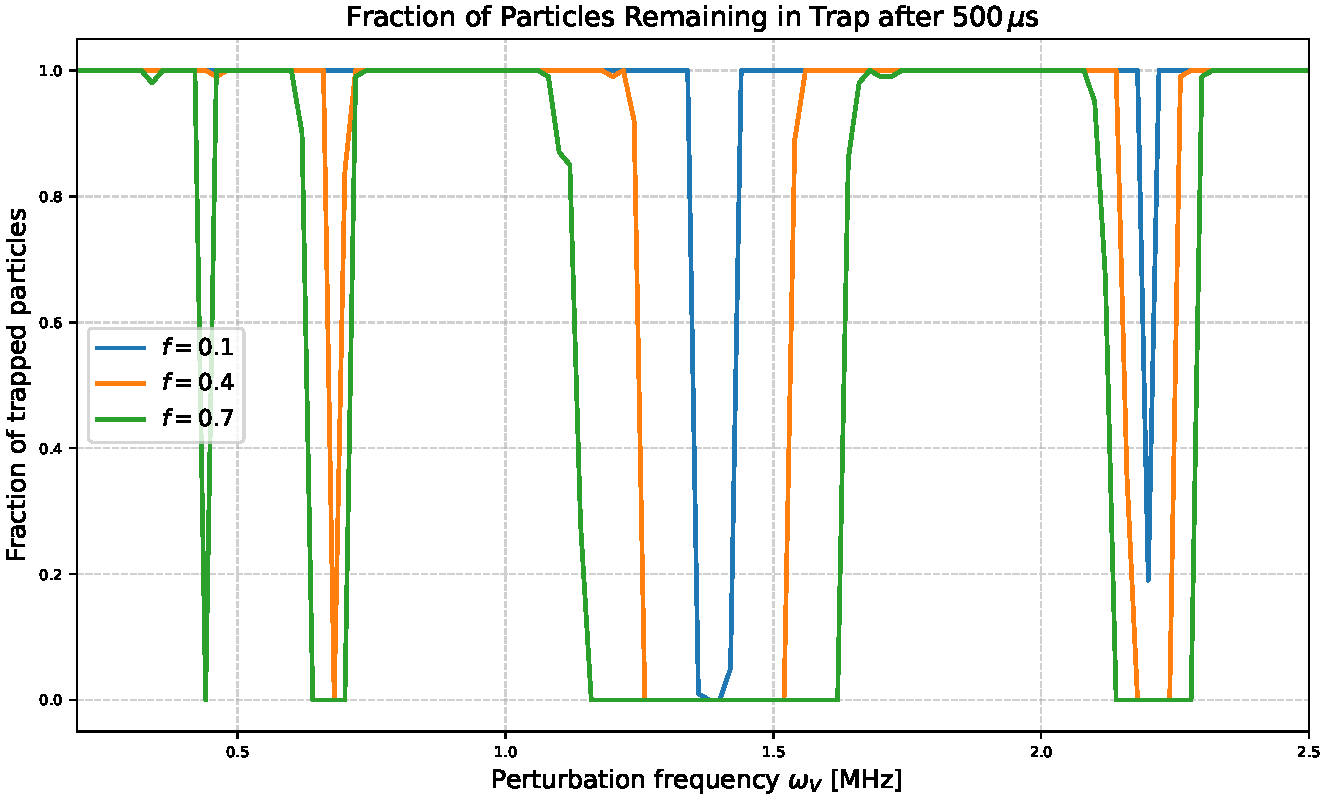
\includegraphics[width=1\linewidth]{Figures/coarse_resonance_sweep.pdf}
    \caption{Coarse sweep across a wide range of $\omega_V$}
    \label{fig:coarse_sweep}
\end{figure}

The results of the coarse analysis are plotted in fig. \ref{fig:coarse_sweep}. As can be observed, at certain perturbation frequencies, the number of remaining trapped particles after the simulation period drops sharply. This can be attributed to the phenomenon of resonance. When the period of particle oscillations within the trap aligns with the period of our harmonic perturbation, the minuscule `nudges' amplify constructively, pushing the particle away from the trap.

This effect is, somewhat predictably, strengthened for larger amplitudes, as indicated by the widening of resonance ranges at higher $f$. Bigger perturbation amplitudes exert greater influence on the particles, leading to more particles escaping at frequencies farther from the exact resonance.

Next, we performed a more detailed analysis around one of the discovered resonance frequencies ($\omega_V\approx1.39$ MHz). We narrowed the exploration window to $\omega_V \in \left[1.0,1.8\right]$ MHz and used a 10-times smaller $d\omega= 0.002$ MHz to increase the resolution. We also performed simulations for scenarios accounting and not accounting for inter-particle interactions (Coulomb). The time step was kept at $dt=0.0125$ $\mu$s due to the significantly increased computational workload in the inter-particle interaction version (the algorithm becomes $\mathcal{O}(n^2)$).

Figures \ref{fig:fine_sweep_inter} and \ref{fig:fine_sweep_nointer} present the results for scenarios with and without inter-particle interactions, respectively. The former is, due to its nature, inherently more chaotic. The random initial state vectors of the particles introduce noise to the picture, which has a more pronounced effect if the particles can interact. The lines in the no-interaction scenario graph are therefore noticeably smoother, but not perfectly smooth either (noise still has an effect). The previously observed behaviour for different perturbation amplitudes also holds in this finer regime -- larger $f$ leads to a broader region of particle escape around the resonant frequency.

\begin{figure}
    \centering
    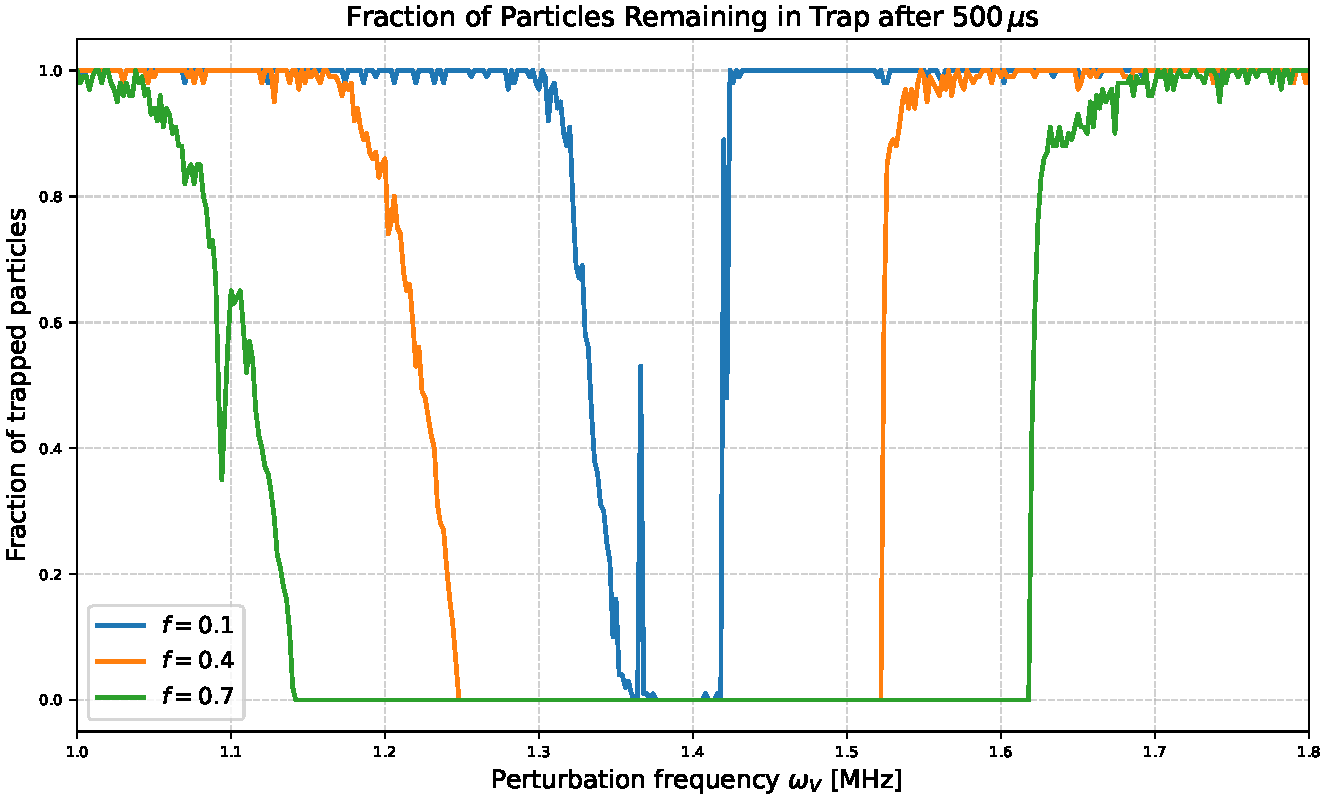
\includegraphics[width=1\linewidth]{Figures/fine_resonance_sweep_inter.pdf}
    \caption{Fine sweep across a narrow range of $\omega_V$, with inter-particle interactions}
    \label{fig:fine_sweep_inter}
\end{figure}

\begin{figure}
    \centering
    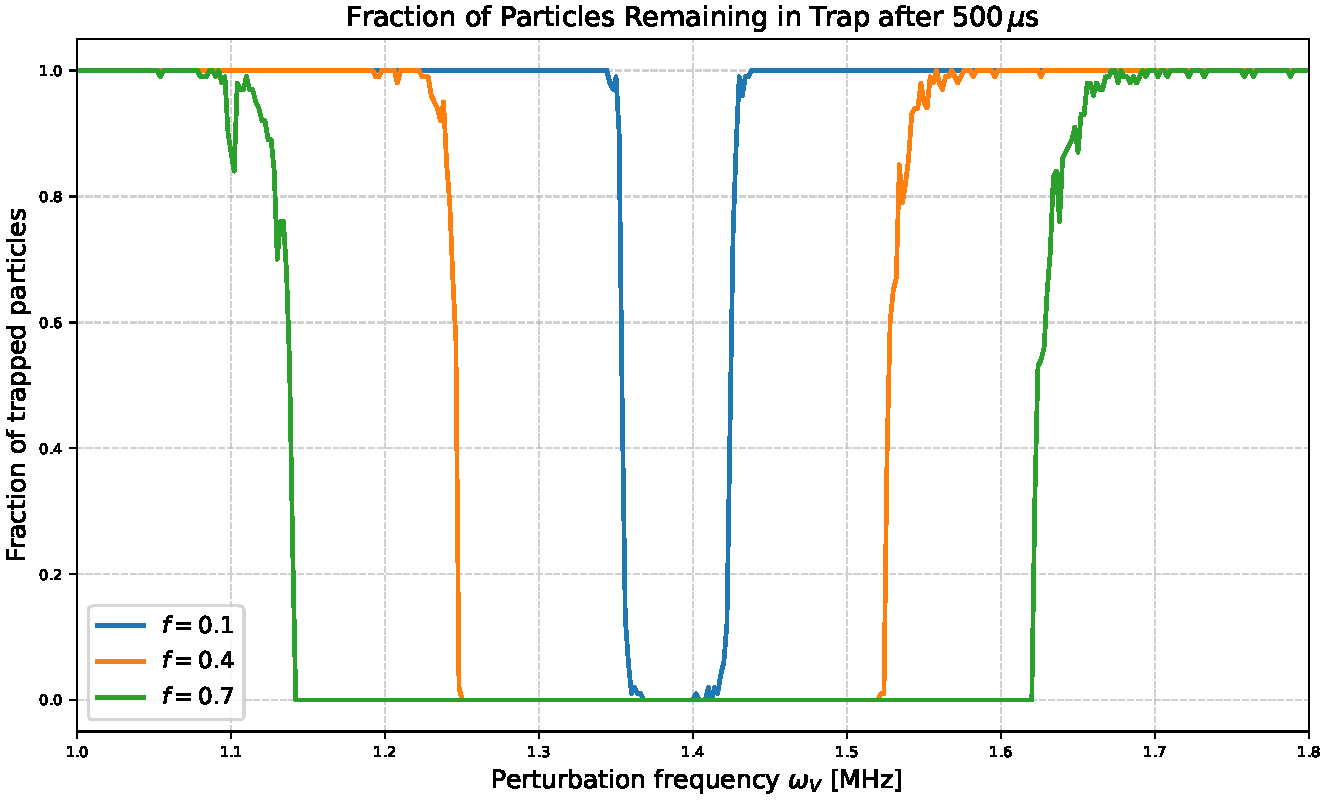
\includegraphics[width=1\linewidth]{Figures/fine_resonance_sweep_nointer.pdf}
    \caption{Fine sweep across a narrow range of $\omega_V$, without inter-particle interactions}
    \label{fig:fine_sweep_nointer}
\end{figure}

In the scenario that accounts for interactions, we also observe that the trap begins to lose particles farther from the resonant frequency. Interestingly, however, the slope is gradual, and the total loss of particles happens at approximately the same frequencies as in the no-interaction case.
% ===========================================
\section{Conclusion}\label{sec:conclusion}
Our results show that the RK4 method with 32000 steps over a $50 \mu s$ can simulate an ideal Penning trap to a final, relative error of $2.31 \cdot 10^{-11}$ in comparison to the analytical solution derived in \cref{sec:penningtrap}.
Furthermore, we found empirical evidence for the global error of the RK4 method to be of order $\mathcal{O}(dt^4)$, which is in line with the theoretical order. In comparison, the less accurate FE method showed a final, relative error of 0.06. 
The introduction of a second particle into the system led to significant coupling between the two particles, as they transferred energy through the Coulomb force. We can clearly see this in Figures \ref{fig:2-particle} and \ref{fig:phase-space-plots}, where the simulated paths and phase spaces of the two particles are plotted.\\
The subsequent analysis of the perturbed case demonstrated the phenomenon of resonance in Penning traps. We conducted an inquiry into the influence of perturbation amplitude and angular frequency on particle loss, identifying the ranges where the effect is most pronounced (around resonant frequencies). We've also shown that an increase in amplitude clearly correlates with the widening of said ranges. The following higher-resolution sweeps showed that including inter-particle forces in the simulation yields noticeably different, noisier results.
Ultimately, these resonance effects expose the inherent instability of the trap under specific time-dependent perturbations.
An applied frequency near the system's resonance leads to the rapid escape of the confined particles, resulting in a complete breakdown of the trap's underlying function. \\
A possible usage of a more specialized numerical method, such as a leapfrog/Verlet algorithm in combination with a Boris push, could lead to more physically sound results\cite{LectureNotes}. This could be especially useful for a larger simulation period, where a more significant energy drift in the RK4 method could occur. \\
The analysis of perturbed Penning traps, although successful, was quite computationally demanding. This necessitated limiting the simulation to 100 particles and choosing a larger time step, which could negatively impact accuracy. The introduction of multithreading or GPU-parallelisation could greatly accelerate these computations, as simulations for separate amplitudes and frequencies constitute independent problems and are therefore trivially parallelisable.



% ===========================================
% \section*{Appendix A}\label{sec:AppendixA}

% An appendix can be useful if there are details you want to include that do not fit in the main text. But if you include an appendix, make sure to explicitly refer to it somewhere in the main text.


% ===========================================
\onecolumngrid
% \bibliographystyle{apalike}
\bibliographystyle{unsrt}
\bibliography{references}


\end{document}
